\documentclass[12pt]{article}
\usepackage[a4paper, total={6in, 8in}]{geometry}
\usepackage{polski}
\usepackage{adjustbox}
\usepackage{pgfplots}
\pgfplotsset{compat=newest}
\usepackage{amsmath}
\usepackage{caption}
\usepackage{url}
\usepackage{hyperref}
\usepackage{adjustbox}
\usepackage{multirow}
\usepackage{titling}

\setlength{\droptitle}{-10em}

\setlength{\parindent}{0pt}
\setlength{\oddsidemargin}{-15pt}
\setlength{\textwidth}{480pt}
\setlength{\textheight}{730pt}

\newcommand{\dpartial}[2]{\frac{\partial #1}{\partial #2}}
\newcommand{\physdpartial}[2]{\left( \dpartial{#1}{#2} \right)^2}
\newcommand{\powfrac}[2]{\left( \frac{#1}{#2} \right)^2}
\newcommand{\powsq}[1]{\left( #1 \right)^{\frac{3}{2}}}

\author{Michał Puchyr, Dawid Chudzicki}
\title{Sprawozdanie z ćwiczenia 48 \\ \textbf{Wyznaczenie stałej plancka na podstawie charakterystyki diody elektroluminescencyjnej}}

\pgfplotsset{scaled x ticks=false}

\begin{document}
\maketitle

\section{Cele ćwiczenia}
\begin{itemize}
    \item Pomiar charakterystyki prądowo-napięciowej diody elektroluminescencyjnej
    w kierunku przewodzenia.
    \item Wyznaczenie długości fali promieniowania emitowanego przez diodę
    elektroluminescencyjną.
    \item Obliczenie stałej Plancka.
\end{itemize}

\section{Wstęp teoretyczny}

\textbf{Stała Plancka} -- jedna z podstawowych stałych fizycznych łącząca energię
fotonów z częstotliwością promieniowania elektromagnetycznego.

Wartość\footnote{do 20 maja 2019 wartość stałej przyjmowana była jako $ h = 6,626070040(81) \times 10^{-34} \ \textrm{J} \cdot \textrm{s} $} stałej Plancka wynosi 

\[ h = 6,62607015 \times 10^{-34} \ \textrm{kg} \cdot \textrm{m}^2 \cdot \textrm{s}^{-1} \]

\textbf{Światło} (wg. terminologii naukowej \textbf{promieniowanie optyczne}) -- jest to promieniowanie podlegające prawom optyki geometrycznej oraz falowej. 
Przyjmuje się, że promieniowanie optyczne obejmuje zakres fal elektromagnetycznych o długości od 100 nm do 1 mm, 
podzielony na trzy zakresy: ultrafiolet, światło widzialne i podczerwień. Wszystkie te zakresy można obserwować i mierzyć, 
używając podobnego zestawu przyrządów, a wyniki tych badań można opracowywać, stosując te same prawa fizyki. 
\medskip

W eksperymencie pomiary były wykonywane na diodzie żółtej (dł. fali od 565 nm do 590 nm) oraz niebieskiej (dł. fali od 450 nm do 485 nm).
\bigskip

Wykaz przyrządów:
\begin{itemize}
    \item Układ zasilający z płynną regulacją napięcia w kierunku przewodzenia i zaporowym
    \item Dioda elektroluminescencyjna
    \item Woltomierz cyfrowy - KEMOT KT890
    \item Amperomierz cyfrowy - SANWA CD771
    \item Monochromator
    \item Detektor fotooporowy
\end{itemize}

\begin{center}
    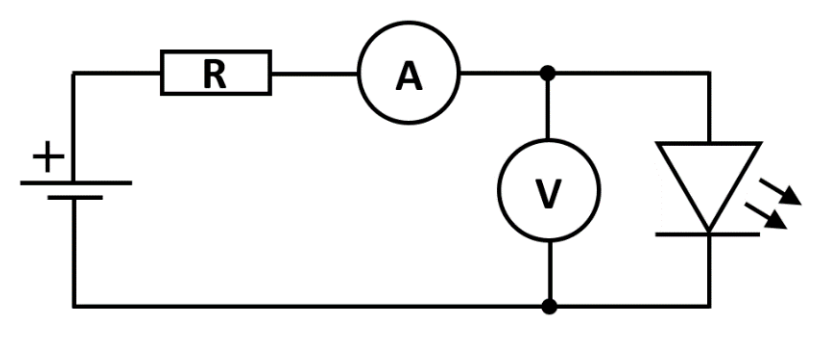
\includegraphics[scale=0.5]{uklad1.png}

    Schemat elektryczny układu do pomiaru charakterystyki prądowo-napięciowej
    diody elektroluminescencyjnej w kierunku przewodzenia

    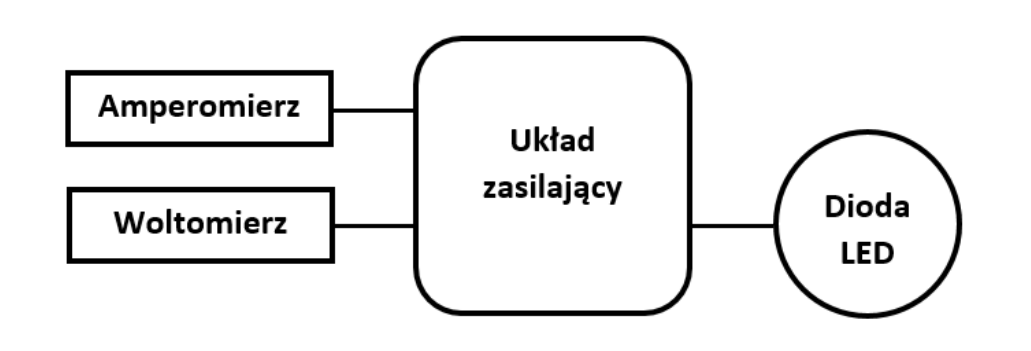
\includegraphics[scale=0.5]{uklad2.png}

    Schemat blokowy układu do pomiaru charakterystyki prądowo-napięciowej
    diody elektroluminescencyjnej
\end{center}

\section{Przykładowe obliczenia}

\subsection{Niepewności mierników}

Niepewność pomiaru napięcia dla woltomierza KEMOT KT890:

Dla zakresu 20 V:

\[ \pm 0,5\% \ \textrm{rdg} + 1 \ \textrm{dgt} = \pm 0,5\% \cdot 0,35 + 1 \cdot 0,01 = \pm 0,01175 \approx \pm 0,012[V] \]

\[ u_b(U) = \frac{\Delta U}{\sqrt{3}} = \frac{0,012}{\sqrt{3}} = 0,00692 \approx 0,007[V] \] \bigskip

Niepewność pomiaru natężenia dla amperomierza SANWA CD771:

Dla zakresu 40 mA:

\[ \pm 1,4\% \ \textrm{rdg} + 3 \ \textrm{dgt} = \pm 1,4\% \cdot 2,51 + 3 \cdot 0,01 = \pm 0,06514 \approx \pm 0,066[mA] \]

\[ u_b(I) = \frac{\Delta I}{\sqrt{3}} = \frac{0,066}{\sqrt{3}} = 0,03810 \approx 0,039[mA] \]

\pagebreak

\subsection{Obliczenia dla pomiarów}

Średnia długość fali:
\[ \overline{\lambda} = \frac{1}{n} \sum\limits_{i = 1}^{n} \lambda_i = \frac{1}{3} \cdot (447 + 444 + 449) =  \frac{1}{3} \cdot 1340 = 446,(6)7 \approx 447[nm] \]
\medskip

Wyznaczenie regresji liniowej:
\begin{center}
    \begin{tikzpicture}
        \begin{axis}[
            xlabel={$I[mA]$},
            ylabel={$U[V]$},
            xmin=0,
            xmax=2.8,
            ymin=0,
            ymax=25,
            xtick={0, 0.5, 1, 1.5, 2, 2.5},
            ytick={0,5,10,15,20,25},
            grid=major,
            grid style={dashed,gray!50},
            width=8cm,
            height=6cm,
            axis lines=middle,
            enlargelimits=0.05,
            tick align=outside,
            legend style={at={(0.5,-0.15)},anchor=north},
            legend cell align=left,
            mark size=2.5pt,
            xticklabel style={
                /pgf/number format/fixed,
                /pgf/number format/precision=5
            },
        ]
        \addplot[red, domain=0:10, dashed, line width=1pt] {62.9*x -135}; \addlegendentry{Regresja liniowa: $y = 62,9x - 135$}
        \addplot[only marks, mark size=1.3, blue, mark=o,error bars/.cd, y dir=both,y explicit] coordinates {
            (0.3500, 0.000) +- (0.0068, 0.018)
            (0.7000, 0.000) +- (0.0078 ,0.018) 
            (1.0500, 0.000) +- (0.0089 ,0.018)
            (1.5000, 0.000) +- (0.011 ,0.018)
            (1.7200, 0.090) +- (0.011 ,0.019)
            (1.9900, 2.510) +- (0.012 ,0.038)
            (2.0300, 3.440) +- (0.012 ,0.046)
            (2.1000, 4.940) +- (0.012 ,0.058)
            (2.1500, 6.810) +- (0.013 ,0.073)
            (2.1800, 7.250) +- (0.013 ,0.076)
            (2.2500, 9.750) +- (0.013 ,0.097)
            (2.3000, 11.920) +- (0.013 ,0.12)
            (2.3500, 14.110) +- (0.013 ,0.14)
            (2.3700, 15.910) +- (0.013 ,0.15)
            (2.4000, 16.580) +- (0.013 ,0.16)
            (2.4300, 18.700) +- (0.013 ,0.17)
            (2.4500, 19.420) +- (0.013 ,0.18)
            (2.4700, 20.500) +- (0.013 ,0.19)
            (2.5000, 22.640) +- (0.013 ,0.21)
            (2.5200, 24.400) +- (0.014 ,0.22)
        };
        \end{axis}
        \end{tikzpicture}
\end{center}

Regresja liniowa wyznaczana była w taki sposób, aby była jak najlepiej dopasowana do prostoliniowej części charakterystyki w kierunku przewodzenia.
Na wykresie zostało przedstawione przykładowe dopasowanie linii regresji liniowej do większości punktów, które można "połączyć" linią prostą.
\smallskip

Wartość napięcia odpowiadającego barierze potencjału (miejsce zerowe regresji liniowej):
\[ U_b = -\frac{b}{a} = -\frac{-134,3}{62,82} = 2,137351 \approx 2,14[V] \]
\medskip

Niepewność obliczenia bariery potencjału:
\[ u(U_b) = \sqrt{ \physdpartial{U_b}{a} \cdot u(a)^2 + \physdpartial{U_b}{b} \cdot u(b)^2 } = \sqrt{ \powfrac{b}{a^2} \cdot u(a)^2 + \powfrac{-1}{a} \cdot u(b)^2 } \]
\[ = \sqrt{ \powfrac{-0,135}{0,0629^2} \cdot 0,0035^2 + \powfrac{-1}{0,0629} + 0,009 } = 0,186375 \approx 0,19[V] \]
\medskip

Obliczenie stałej Plancka:
\[ h = \frac{e}{c} \lambda U_b = \frac{1,6 \cdot 10^{-19}}{299792458} \cdot 447 \cdot 10^{-9} \cdot 2,14 = 6,6814222 \cdot 10^{-34} \approx 6,69 \cdot 10^{-34} \ [\textrm{kg} \cdot \textrm{m}^2 \cdot \textrm{s}^{-1}] \]
\medskip

gdzie:
\begin{itemize}
    \item e -- ładunek elektryczny elementarny
    \item c -- prędkość światła w próżni
\end{itemize}
\medskip

Niepewność obliczenia stałej Plancka:
\[ u_c(h) = \frac{e}{c} \sqrt{ U_b^2 \cdot u(\lambda)^2 + \lambda^2 \cdot u(U_b)^2 } = 5,33 \cdot 10^{-28} \sqrt{ 2,14^2 \cdot (10 \cdot 10^{-9})^2 + (585^2 \cdot 0,19 \cdot 10^{-9})^2 } \]
\[ = 0,61 \cdot 10^{-34} \ [\textrm{kg} \cdot \textrm{m}^2 \cdot \textrm{s}^{-1}] \]

\pagebreak

\section{Pomiary układów}

\subsection{Pomiary długości fali}

\begin{table}[!htb]
    \begin{center}
        \begin{minipage}{.49\linewidth}
            \centering
            \caption*{Zmierzone długości fali dla diody żółtej}
            \begin{tabular}{|c|c|c|c|} \hline
                Lp. & $\lambda$[nm] & u($\lambda$)[nm] & $\overline{\lambda}$[nm] \\ \hline
                1 & 585 & 10 & \multirow{3}{*}{585} \\ \cline{1-3} 
                2 & 585 & 10 &  \\ \cline{1-3} 
                3 & 585 & 10 &  \\ \hline
            \end{tabular}
        \end{minipage}
        \begin{minipage}{.49\linewidth}
            \centering
            \caption*{Zmierzone długości fali dla diody niebieskiej}
            \begin{tabular}{|c|c|c|c|} \hline
                Lp. & $\lambda$[nm] & u($\lambda$)[nm] & $\overline{\lambda}$[nm] \\ \hline
                1 & 447 & 10 & \multirow{3}{*}{447} \\ \cline{1-3} 
                2 & 444 & 10 &  \\ \cline{1-3} 
                3 & 449 & 10 &  \\ \hline
            \end{tabular}
        \end{minipage}
    \end{center}
\end{table}

\subsection{Dioda niebieska}

\begin{center}
    \begin{tikzpicture}
        \begin{axis}[
            xlabel={$I[mA]$},
            ylabel={$U[V]$},
            xmin=0,
            xmax=2.8,
            ymin=0,
            ymax=25,
            xtick={0, 0.5, 1, 1.5, 2, 2.5},
            ytick={0,5,10,15,20,25},
            grid=major,
            grid style={dashed,gray!50},
            width=15cm,
            height=11cm,
            axis lines=middle,
            enlargelimits=0.05,
            tick align=outside,
            legend style={at={(0.5,-0.15)},anchor=north},
            legend cell align=left,
            mark size=2.5pt,
            xticklabel style={
                /pgf/number format/fixed,
                /pgf/number format/precision=5
            },
        ]
        \addplot[red, domain=0:10, dashed, line width=1.5pt] {62.9*x -135}; \addlegendentry{Regresja liniowa: $y = 62,9x - 135$}
        \addplot[only marks, blue, mark=o,error bars/.cd, y dir=both,y explicit] coordinates {
            (0.3500, 0.000) +- (0.0068, 0.018)
            (0.7000, 0.000) +- (0.0078 ,0.018) 
            (1.0500, 0.000) +- (0.0089 ,0.018)
            (1.5000, 0.000) +- (0.011 ,0.018)
            (1.7200, 0.090) +- (0.011 ,0.019)
            (1.9900, 2.510) +- (0.012 ,0.038)
            (2.0300, 3.440) +- (0.012 ,0.046)
            (2.1000, 4.940) +- (0.012 ,0.058)
            (2.1500, 6.810) +- (0.013 ,0.073)
            (2.1800, 7.250) +- (0.013 ,0.076)
            (2.2500, 9.750) +- (0.013 ,0.097)
            (2.3000, 11.920) +- (0.013 ,0.12)
            (2.3500, 14.110) +- (0.013 ,0.14)
            (2.3700, 15.910) +- (0.013 ,0.15)
            (2.4000, 16.580) +- (0.013 ,0.16)
            (2.4300, 18.700) +- (0.013 ,0.17)
            (2.4500, 19.420) +- (0.013 ,0.18)
            (2.4700, 20.500) +- (0.013 ,0.19)
            (2.5000, 22.640) +- (0.013 ,0.21)
            (2.5200, 24.400) +- (0.014 ,0.22)
        };
        \end{axis}
        \end{tikzpicture}
    
        \textbf{Wykres zależności napięcia od natężenia dla niebieskiej diody}
\end{center}


\begin{table}[]
    \caption*{Pomiary i obliczone wartości dla układu z diodą niebieską}
        \begin{tabular}{|l|l|l|l|l|c|c|c|c|c|c|c|} \hline
        Lp. & U[V] & u(U)[V] & I[mA] & u(I)[mA] & U\textsubscript{b}[V] & u(U\textsubscript{b})[V] & h[kg $\cdot$ m$^2 \cdot$ s$^{-1}$] & u(h)[kg $\cdot$ m$^2 \cdot$ s$^{-1}$] \\ \hline
        1 & 0,3500 & 0,0068 & 0,000 & 0,018 & \multirow{20}{*}{2,14} & \multirow{20}{*}{0,19} & \multirow{20}{*}{$6,69 \cdot 10^{-34}$} & \multirow{20}{*}{$0,61 \cdot 10^{-34}$} \\ \cline{1-5}
        2 & 0,7000 & 0,0078 & 0,000 & 0,018 &  &  &  &  \\ \cline{1-5}
        3 & 1,0500 & 0,0089 & 0,000 & 0,018 &  &  &  &  \\ \cline{1-5}
        4 & 1,500 & 0,011 & 0,000 & 0,018 &  &  &  &  \\ \cline{1-5}
        5 & 1,720 & 0,011 & 0,090 & 0,019 &  &  &  &  \\ \cline{1-5}
        6 & 1,990 & 0,012 & 2,510 & 0,038 &  &  &  &  \\ \cline{1-5}
        7 & 2,030 & 0,012 & 3,440 & 0,046 &  &  &  &  \\ \cline{1-5}
        8 & 2,100 & 0,012 & 4,940 & 0,058 &  &  &  &  \\ \cline{1-5}
        9 & 2,150 & 0,012 & 6,810 & 0,073  &  &  &  &  \\ \cline{1-5}
        10 & 2,180 & 0,013 & 7,250 & 0,076 &  &  &  &  \\ \cline{1-5}
        11 & 2,250 & 0,013 & 9,750 & 0,097 &  &  &  &  \\ \cline{1-5}
        12 & 2,300 & 0,013 & 11,92 & 0,12 &  &  &  &  \\ \cline{1-5}
        13 & 2,350 & 0,013 & 14,11 & 0,14 &  &  &  &  \\ \cline{1-5}
        14 & 2,370 & 0,013 & 15,91 & 0,15 &  &  &  &  \\ \cline{1-5}
        15 & 2,400 & 0,013 & 16,58 & 0,16 &  &  &  &  \\ \cline{1-5}
        16 & 2,430 & 0,013 & 18,70 & 0,17 &  &  &  &  \\ \cline{1-5}
        17 & 2,450 & 0,013 & 19,42 & 0,18 &  &  &  &  \\ \cline{1-5}
        18 & 2,470 & 0,013 & 20,50 & 0,19 &  &  &  &  \\ \cline{1-5}
        19 & 2,500 & 0,013 & 22,64 & 0,21 &  &  &  &  \\ \cline{1-5}
        20 & 2,520 & 0,014 & 24,40 & 0,22 &  &  &  &  \\ \hline
        \end{tabular}
\end{table}

\subsection{Dioda żółta}

\begin{center}
    \begin{tikzpicture}
        \begin{axis}[
            xlabel={$I[mA]$},
            ylabel={$U[V]$},
            xmin=0,
            xmax=3.5,
            ymin=0,
            ymax=20,
            xtick={0, 0.5, 1, 1.5, 2, 2.5, 3.0, 3.5},
            ytick={0,5,10,15,20},
            grid=major,
            grid style={dashed,gray!50},
            width=15cm,
            height=11cm,
            axis lines=middle,
            enlargelimits=0.05,
            tick align=outside,
            legend style={at={(0.5,-0.15)},anchor=north},
            legend cell align=left,
            mark size=2.5pt,
            xticklabel style={
                /pgf/number format/fixed,
                /pgf/number format/precision=5
            },
        ]
        \addplot[red, domain=0:10, dashed, line width=1.5pt] {61.0*x -171}; \addlegendentry{Regresja liniowa: $y = 61,0x - 171$}
        \addplot[only marks, blue, mark=o,error bars/.cd, y dir=both,y explicit] coordinates {
            (0.5000, 0.000) +- (0.0058, 0.018)
            (1.0000, 0.000) +- (0.0058, 0.018)
            (1.5000, 0.000) +- (0.0058, 0.018)
            (2.0000, 0.000) +- (0.0060, 0.018)
            (2.5000, 0.050) +- (0.0060, 0.018)
            (2.6500, 0.740) +- (0.0080, 0.024)
            (2.7000, 1.330) +- (0.0100, 0.029)
            (2.7300, 1.960) +- (0.0120, 0.034)
            (2.7700, 2.660) +- (0.0140, 0.039)
            (2.8000, 3.350) +- (0.0160, 0.045)
            (2.8300, 4.280) +- (0.0190, 0.052)
            (2.8600, 5.300) +- (0.0220, 0.070)
            (2.8900, 6.490) +- (0.0250, 0.070)
            (2.9200, 7.860) +- (0.0290, 0.090)
            (2.9500, 9.350) +- (0.0330, 0.100)
            (2.9800, 11.060) +- (0.0380, 0.110)
            (3.0100, 12.860) +- (0.0430, 0.130)
            (3.0400, 14.770) +- (0.0490, 0.140)
            (3.0700, 17.080) +- (0.0560, 0.160)
            (3.0900, 18.720) +- (0.0600, 0.170)
        };
        \end{axis}
        \end{tikzpicture}
    
        \textbf{Wykres zależności napięcia od natężenia dla żółtej diody}
\end{center}

\begin{table}[]
    \caption*{Pomiary i obliczone wartości dla układu z diodą żółtą}
    \begin{tabular}{|l|l|l|l|l|c|c|c|c|} \hline
        Lp. & U & u(U) & I[mA] & u(I)[mA] & U\textsubscript{b}[V] & u(U\textsubscript{b})[V] & h[kg $\cdot$ m$^2 \cdot$ s$^{-1}$] & u(h)[kg $\cdot$ m$^2 \cdot$ s$^{-1}$] \\ \hline
        1 & 0,5000 & 0,0073 & 0,000 & 0,018 & \multirow{20}{*}{2,80} & \multirow{20}{*}{0,16} & \multirow{20}{*}{$6,68 \cdot 10^{-34}$} & \multirow{20}{*}{$0,41 \cdot 10^{-34}$} \\ \cline{1-5}
        2 & 1,0000 & 0,0087 & 0,000 & 0,018 &  &  &  &  \\ \cline{1-5}
        3 & 1,5000 & 0,0102 & 0,000 & 0,018 &  &  &  &  \\ \cline{1-5}
        4 & 2,000 & 0,012 & 0,000 & 0,018 &  &  &  &  \\ \cline{1-5}
        5 & 2,500 & 0,013 & 0,050 & 0,018 &  &  &  &  \\ \cline{1-5}
        6 & 2,650 & 0,014 & 0,740 & 0,024 &  &  &  &  \\ \cline{1-5}
        7 & 2,700 & 0,014 & 1,330 & 0,029 &  &  &  &  \\ \cline{1-5}
        8 & 2,730 & 0,014 & 1,960 & 0,034 &  &  &  &  \\ \cline{1-5}
        9 & 2,770 & 0,014 & 2,660 & 0,039 &  &  &  &  \\ \cline{1-5}
        10 & 2,800 & 0,014 & 3,350 & 0,045 &  &  &  &  \\ \cline{1-5}
        11 & 2,830 & 0,014 & 4,280 & 0,052 &  &  &  &  \\ \cline{1-5}
        12 & 2,860 & 0,015 & 5,30 & 0,07 &  &  &  &  \\ \cline{1-5}
        13 & 2,890 & 0,015 & 6,49 & 0,07 &  &  &  &  \\ \cline{1-5}
        14 & 2,920 & 0,015 & 7,86 & 0,09 &  &  &  &  \\ \cline{1-5}
        15 & 2,950 & 0,015 & 9,35 & 0,10 &  &  &  &  \\ \cline{1-5}
        16 & 2,980 & 0,015 & 11,06 & 0,11 &  &  &  &  \\ \cline{1-5}
        17 & 3,010 & 0,015 & 12,86 & 0,13 &  &  &  &  \\ \cline{1-5}
        18 & 3,040 & 0,015 & 14,77 & 0,14 &  &  &  &  \\ \cline{1-5}
        19 & 3,070 & 0,015 & 17,08 & 0,16 &  &  &  &  \\ \cline{1-5}
        20 & 3,090 & 0,015 & 18,72 & 0,17 &  &  &  &  \\ \hline
    \end{tabular}
\end{table}

\section{Wnioski}

Przy pomocy pomiarów oraz wykonanych obliczeń udało się wyznaczyć przybliżenie stałej Plancka.

Udało się również wyznaczyć długości fali promieniowania emitowanego przez diody elektroluminescencyjne,
które pokrywają się z wartościami faktycznymi.

Wpływ na niewielką rozbieżność między faktyczną wartością stałej a tą wyznaczonej z eksperymentu 
ma niedokładność mierników oraz niedoskonałość w ocenie koloru przez ludzkie oko. \bigskip

Porównując wartość stałej plancka 
\[ h = 6,62607015 \times 10^{-34} \ \textrm{kg} \cdot \textrm{m}^2 \cdot \textrm{s}^{-1} \]
do tych, które zostały wyznaczone przy pomocy pomiarów i obliczeń
\[ h = (6,69 \pm 0,61) \times 10^{-34} \ \textrm{kg} \cdot \textrm{m}^2 \cdot \textrm{s}^{-1} \] 
\[ h = (6,68 \pm 0,41) \times 10^{-34} \ \textrm{kg} \cdot \textrm{m}^2 \cdot \textrm{s}^{-1} \] 

można stwierdzić, że eksperyment został pomyślnie przeprowadzony.

\section{Bibliografia}

\begin{itemize}
    \item \url{https://pl.wikipedia.org/wiki/Stała_Plancka}
    \item \url{https://pl.wikipedia.org/wiki/Światło}
\end{itemize}

\end{document}